%%*****************************************************************************
%% $Id: extex-users.tex,v 1.1 2005/05/29 22:00:43 gene Exp $
%%*****************************************************************************
%% Author: Gerd Neugebauer
%%-----------------------------------------------------------------------------
\documentclass[12pt,div12,a4paper]{scrbook}

\usepackage[latin1]{inputenc}
\usepackage{booktabs}
\usepackage{listings}
\usepackage{graphicx,color}
\usepackage[colorlinks=true]{hyperref}

\providecommand*{\ExTeX}{\ifx\texorpdfstring\undefined
  \textrm{% the logo comes always with serifs
    \ensuremath{\textstyle\varepsilon_{\kern-0.15em\mathcal{X}}}%
    \kern-.15em\TeX}%
  \else\texorpdfstring{%
  \textrm{% the logo comes always with serifs
    \ensuremath{\textstyle\varepsilon_{\kern-0.15em\mathcal{X}}}%
    \kern-.15em\TeX
  }}{ExTeX}%
  \fi
}

\lstloadlanguages{TeX}
\lstset{language=TeX,%
  basicstyle=\tt,%
  keywordstyle=\bf,%
  morekeywords={\namespace,\export,\import}%,
  %labelstyle=\sf\tiny,%
  %labelstep=1,%
  %labelsep=5pt,%
  %indent=12pt%
}
\lstset{language=Java,%
  basicstyle=\tt,%
  keywordstyle=\bf,%
  morekeywords={}
}


\newenvironment{abstract}{\begin{quotation}}{\end{quotation}}

\title{ExTeX User's Guide}
\author{Gerd Neugebauer}
%\date{}

\begin{document}%%%%%%%%%%%%%%%%%%%%%%%%%%%%%%%%%%%%%%%%%%%%%%%%%%%%%%%%%%%%%%%

\begin{titlepage}
  \begin{center}
  \vspace*{1pt}
  \vfill
  
\includegraphics[width=\textwidth]{ExTeX-splash.png}
  \vfill
  \textsf{\Huge User's Guide}
  \vfill
  \textsf{\Large Version 0.1}
  \vfill
  \textsf{\large Gerd Neugebauer}
  \vfill
  \vfill
%\maketitle

  \begin{abstract}
    This document describes some basic steps to develop and test \ExTeX.
    It is meant for newcomers to the project or people who want to
    evaluate \ExTeX.
  \end{abstract}
  \end{center}
\newpage
\footnotesize
\copyright\ 2005 The \ExTeX\ Group and individual authors listed below 

\ExTeX{} is free software; you can redistribute it and/or modify it
under the terms of the \href{LGPL.html}{LibraryGNU General Public
  License} as published by the Free Software Foundation; either
version 1, or (at your option) any later version.

\ExTeX{} is distributed in the hope that it will be useful, but
WITHOUT ANY WARRANTY; without even the implied warranty of
MERCHANTABILITY or FITNESS FOR A PARTICULAR PURPOSE.  See the
\href{LGPL.html}{Library GNU General Public License} for more details.

You should have received a copy of the \href{LGPL.html}{Library GNU
  General Public License} along with this documentation; see the file
\href{LGPL.html}{LICENSE.txt}.  If not, write to the Free Software
Foundation, 675 Mass Ave, Cambridge, MA 02139, USA. 
\vfill

\noindent
Gerd Neugebauer\\
Im Lerchelsb\"ohl 5\\
64521 Gro\ss-Gerau (Germany)\smallskip\par\noindent WWW:
\url{http://www.gerd-neugebauer.de/}
\smallskip\par\noindent Net: \href{mailto://gene@gerd-neugebauer.de}{gene@gerd-neugebauer.de}

\end{titlepage}


\newpage
\tableofcontents
\newpage

\chapter{Introduction}

\ExTeX{} aims at providing a high-quality typesetting system. The
development of \ExTeX\ has been inspired by the experiences with \TeX.


\section{Web Site}

There is a web site devoted to \ExTeX. This web site can be reached
via the URL

\begin{quotation}
  \url{http://www.extex.org}
\end{quotation}


\section{Mailing Lists}

If you are ready to try \ExTeX{} you might as well want to join a
mailing list to get in contact with the community.

\begin{quotation}
  \url{http://www.dante.de/listman/extex}
\end{quotation}


\chapter{Getting Started}

In this chapter we describe the steps you can take to get \ExTeX\ up
and running. We try to use as few as possible premises. Thus it should
be not too hard to get started.

\section{Prerequisites}

\subsection{Java}

You need to have Java 1.4.2 or later installed on your system. You can
get Java for a several systems directly from \url{java.sun.com}.
Download and install it accoring to the installation instructions for
your environment.

To check that you have an appropriate Java on your path you can use
the command \texttt{java} with the argument \texttt{-version}. This
can be seen in the following listing:

{\small
\begin{lstlisting}{}
> java -version
java version "1.4.2_06"
Java(TM) 2 Runtime Environment, Standard Edition (build 1.4.2_06-b03)
Java HotSpot(TM) Client VM (build 1.4.2_06-b03, mixed mode)
>
\end{lstlisting}}


\subsection{TEXMF}

If you want to use more than the pure \TeX\ engine fonts and macros
can be inherited from texmf tree.



\section{Getting \ExTeX}

The sources of \ExTeX\ are stored in a RCS repository. To access this
repository you need access to the internet and RCS installed in some
way.

The coordinates of the repository are:
\medskip

\begin{tabular}{ll}\toprule
  Connection type: & \texttt{pserver}			\\
  User:		   & \texttt{anonymous}			\\
  Host:		   & \texttt{cvs.extex.berlios.de}	\\
  Location:	   & \texttt{/cvsroot/extex}		\\
  Module:	   & \texttt{ExTeX}			\\\bottomrule
\end{tabular}
\bigskip

We assume here that you have access to cvs on the command line. This
can be either a shell on a Unix-like system or somethng like cygwin on
Windows. We also assume that you have direct connection to the internet.

First we create a directory where the sources are stored:
\begin{lstlisting}{}
> mkdir ExTeX
\end{lstlisting}

Next we change the current directory to this base directory:
\begin{lstlisting}{}
> cd ExTeX
\end{lstlisting}

Now we log into the CVS repository. This login uses an anonymous
account. This enables us to download the sources but not to commit any
changes. The committing is restricted to members of the \ExTeX{} team.
\begin{lstlisting}{}
> cvs -d:pserver:anonymous@cvs.extex.berlios.de/cvsroot/extex login
\end{lstlisting}

Finally we can check out the sources:
\begin{lstlisting}{}
> cvs -d:pserver:anonymous@cvs.extex.berlios.de/cvsroot/extex co ExTeX
\end{lstlisting}

This command shows a lot of output. At the end the current directory
is filled with a lot of files and directories.

\section{Installing \ExTeX\ from the Command Line}

To install you can use the build script provided in the \ExTeX{}
base directory.

\begin{lstlisting}{}
> build -Dinstall.dir=/usr/local/share/ExTeX install
\end{lstlisting}

Now you can forget the source directory. It is not needed any more
unless you are debugging or developing \ExTeX{} extensions.

\section{Installing \ExTeX\ with the Installer}

You can make use of the installer of \ExTeX. To use the installer you
have to create it from the sources. All you need for this step is
contaoned in the source distribution.

\begin{lstlisting}{}
> build installer
\end{lstlisting}

As a result the file \texttt{ExTeX-setup.jar} is created in the
directory \texttt{target}. This file is a self-contained installer.
You can start the installer with the following command line:

\begin{lstlisting}{}
> java -jar target/ExTeX-setup.jar
\end{lstlisting}

On windows with a properly installed Java you can also start the
installer by double-clicking \texttt{ExTeX-setup.jar} in the Explorer.

\begin{figure}[htp]
  \centering
  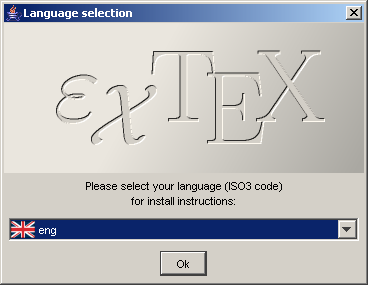
\includegraphics[width=.5\textwidth]{inst1.png}
  \caption{The Language Selection in the Installer}
  \label{fig:inst1}
\end{figure}

The installer provides a graphical user interface with a wizard
guiding you through the installation process. The first dialog is
shown in figure~\ref{fig:inst1}. As you can see you can select one of
several languages for the installation process. Currently the
languages English and German are supported. There might be some more
at the time you are performing the installation.

Note that the internationalization covers the installer only. \ExTeX\
can be run under different language environments as well. This is
controlled by a setting at run-time. Currently only an English
language binding for \ExTeX\ is provided.


\chapter{Configuring \ExTeX}

The behaviour of \ExTeX\ can be influenced via command line arguments
and configuration files.


\section{Startup Files}

Whenever \ExTeX\ starts it looks for startup files named
\texttt{.extex}. This file is sought in the user's home directory in
in the current directory. The settings in the current directoy
overwrite the settings from the user's home directory. Those in turn
overwrite the built-in settings.


\section{Configuration Files}

Configuration files of another kind contain the assembly instructions
for \ExTeX. Those files can be used to provide additional features in
\ExTeX. 


\chapter{Running \ExTeX}

Currently \ExTeX\ can be run from the command line. In this respect it
is more or less identical to \TeX\ and can be used as a plug-in
replacement.

\section{Command Line Parameters}



\section{Creating Formats}






\end{document}%%%%%%%%%%%%%%%%%%%%%%%%%%%%%%%%%%%%%%%%%%%%%%%%%%%%%%%%%%%%%%%%%
%
% Local Variables: 
% mode: latex
% TeX-master: nil
% End: 
